Un diagramma di fase (o diagramma di stato) è un particolare diagramma cartesiano sperimentale riferito ad una sostanza pura o ad una miscela, che rappresenta lo stato del sistema termodinamico in esame al variare di due o più coordinate termodinamiche (temperatura, pressione, volume, composizione chimica (frazione molare)).

\subsection{Diagramma di fase per singole speci chimiche}

\begin{figure}[htp]
    \centering
    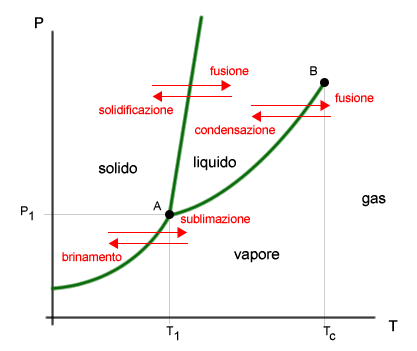
\includegraphics[width=10cm]{immagini/diagramma_di_stato.png}
\end{figure}

Tale grafico è inerente ad una singola specie chimica, ed ha temperatura sulle ascisse e la pressione sulle ordinate. Siccome non riguarda una soluzione non avremo una frazione molare. In esso troviamo le fasi e la loro esistenza, cioè le regioni (che corrispondono a coppie di valori di temperatura e pressione) che permettono l'esistenza di tale fase.

Sulle linee tratteggiate, dette \textbf{confini di fase}, abbiamo coesistenza di due fasi. Laddove sono presenti più di una fase insieme si parla di equilibrio eterogeneo, il quale resta in equilibrio quando non varia il numero di fasi coesistenti in esso.

Il punto di intersezione delle linee di coesistenza è detto \textbf{punto triplo}, in cui si ha la coesistenza di tutte e tre le fasi.

In che modo possiamo muoverci lungo tale diagramma (che corrisponde a variare pressione e temperatura), pur mantenendo lo stesso stato di partenza?

\begin{itemize}
    \item Se ci troviamo in una delle cosiddette regioni di esistenza, ad esempio quella dello stato solido, possiamo variare indipendemente pressione e temperatura entro un certo limite restando nel medesimo stato. Poiché le due variabili sono indipendenti, si dice che tali regioni sono bi-varianti;
    \item Se invece ci troviamo sulle linee non possiamo variare pressione e temperatura indipendentemente l'una dall'altra: la variazione di una delle due determinerà automaticamente la variazione dell'altra, altrimenti la coesistenza di due fasi non verrà preservata. Quindi lungo le linee una delle due variabili è indipendenti mentre l'altra è dipendente, per cui esse sono dette mono-varianti;
    \item 
    Se infine ci troviamo sul punto triplo non possiamo variare né la pressione né la temperatura, altrimenti perderemmo la coesistenza dei tre stati e quindi l'equilibrio eterogeneo. Per questo motivo esso è detto zero-variante.
\end{itemize}

\subsubsection{Diagramma di stato dell'acqua}
Consideriamo il diagramma di stato dell'acqua.

Abbiamo detto che esso è un diagramma sperimentale. Come si fanno le misure?

Immaginiamo di avere un cilindro munito di pistone in cui è preventivamente fatto il vuoto e dentro di esso mettiamo dell'acqua. Il sistema è tale da permetterci di misurare la temperatura interne e la tensione di vapore.

Ciò che si fa è fissare delle temperature scelte da noi (si parte da basse temperature) e leggere le corrispondenti tensioni di vapore. Dopodiché si va a vedere come varia la temperatura di fusione del ghiaccio al variare della pressione esterna esercitata, cioè scegliamo noi la pressione.

Ci si accorge che all'aumentare della pressione il ghiaccio fonde a temperature via via sempre più basse.

Attenzione! Sono due esperimenti diversi. Nel primo si misura la tensione di vapore dell'acqua al variare della sua temperatura, nel secondo si misura la temperatura di fusione del ghiaccio al variare della pressione esterna esercitata. Cioè prima variamo la temperatura e misuriamo la pressione, dopodiché variamo la pressione e misuriamo la temperatura.

Riportando le misure su un grafico otteniamo il diagramma:

\begin{figure}[htp]
    \centering
    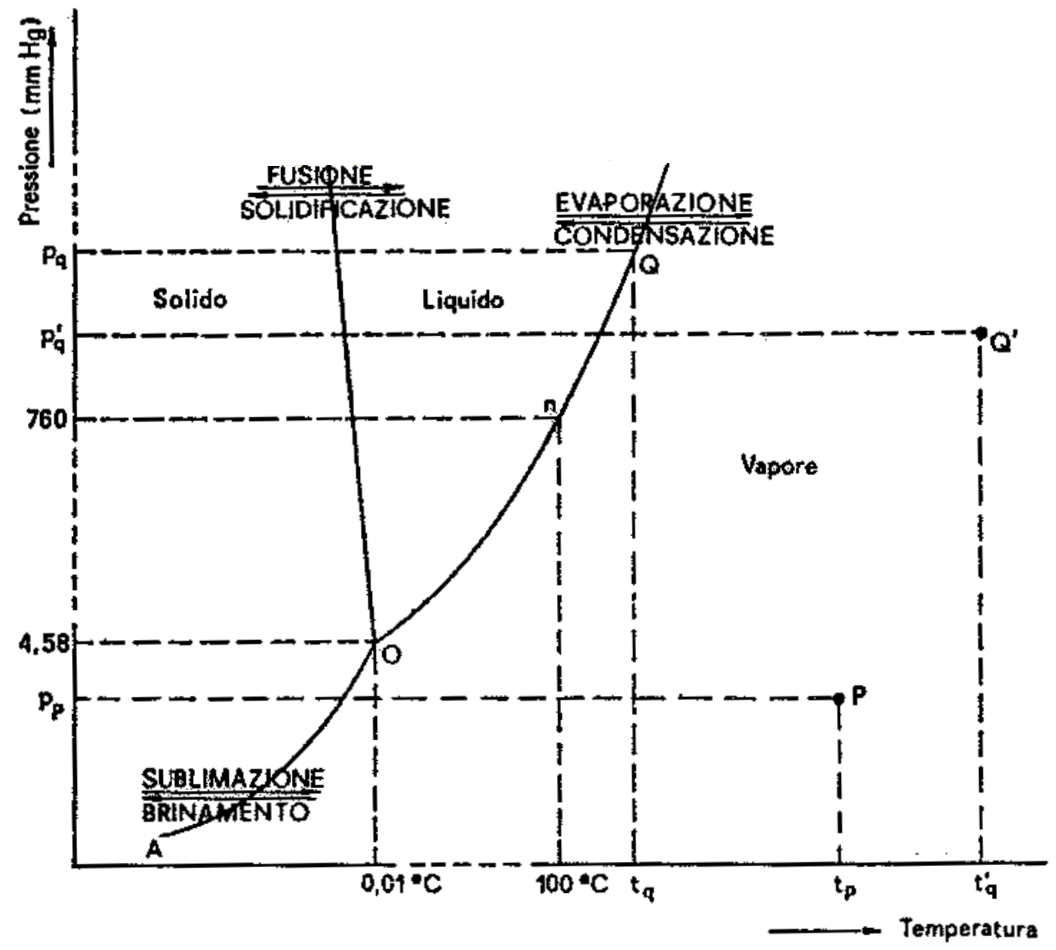
\includegraphics[width=10cm]{immagini/diagramma_di_stato_acqua.png}
\end{figure}

L'acqua è l'unica sostanza che, al diminuire della temperatura, aumenta in volume. Ciò nel diagramma si traduce con una pendenza negativa della linea che separa solido e liquido. Tutti gli altri diagrammi infatti hanno tale linea con pendenza positiva.

Nei fatti a circa 4° C l'acqua ha la sua massima densità. Il motivo è che quando l'acqua viene raffreddata vengono favoriti i legami a idrogeno. Si realizza quindi un sistema esteso di interazioni e per mantenerle l'acqua aumenta di volume.

Il punto triplo dell'acqua si ha a 0.01° C, temperatura alla quale l'acqua esercita una tensione di vapore di 4.58 torr. In queste condizioni si ha coesistenza di acqua solida, liquida e vaporea.
\subsubsection{Diagramma di stato per CO$_2$}

Vediamo ora un esempio in cui il confine di fase tra solido e liquido ha pendenza positiva: il diagramma di stato dell'anidride carbonica. Esso si ottiene con lo stesso metodo sperimentale sopra descritto.

\begin{figure}[htp]
    \centering
    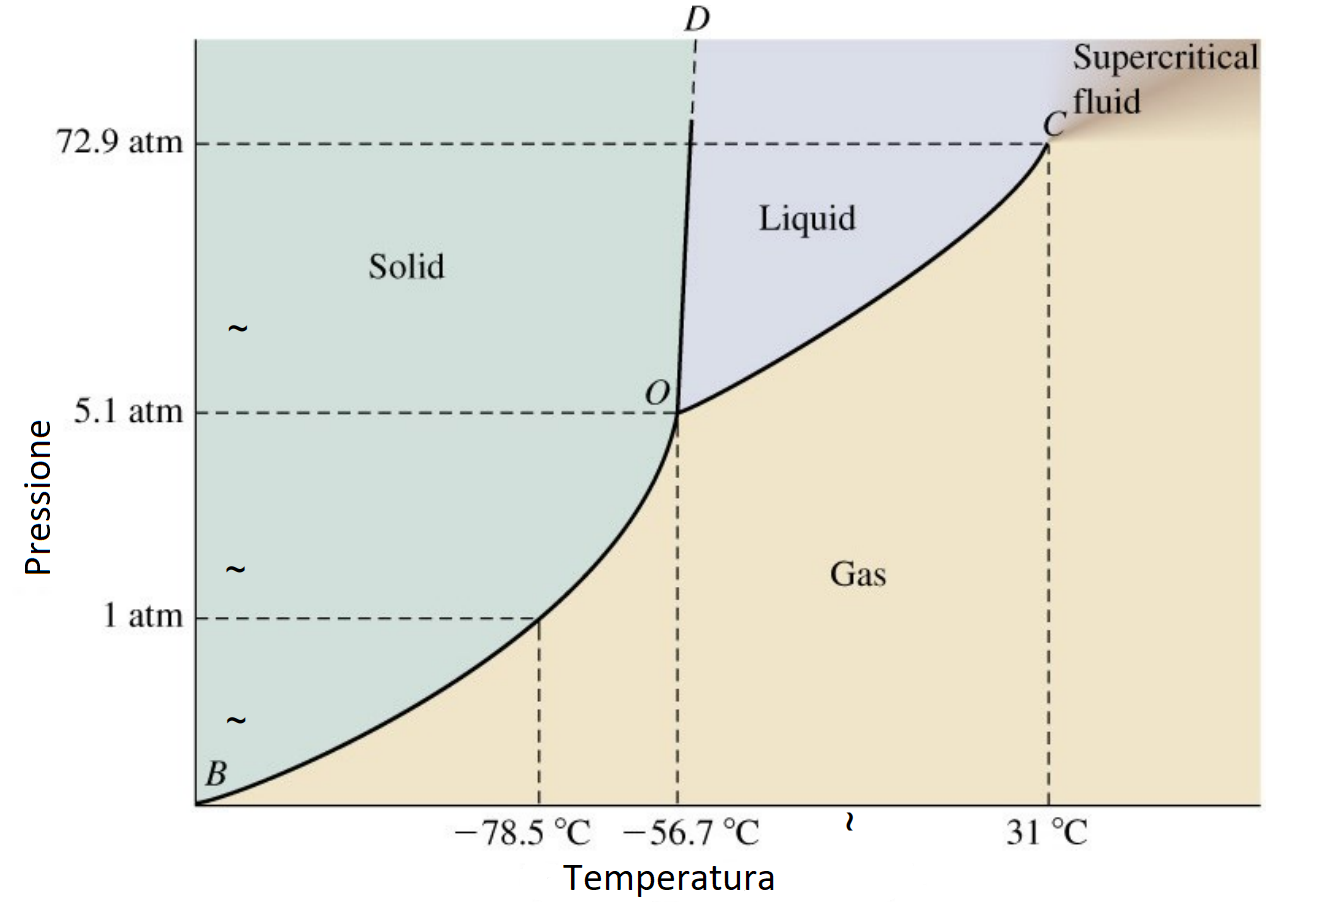
\includegraphics[width=12cm]{immagini/diagramma_di_stato_CO2.png}
\end{figure}

L'anidride carbonica solidifica facilmente, e infatti si ha una pendenza ripida, stavolta però sarà positiva.

Il punto triplo si trova a -56.7° C e 5.1 atm.

\subsection{Diagramma di fase per soluzioni}
\subsubsection{Diagramma di fase della granita}

\begin{figure}[htp]
    \centering
    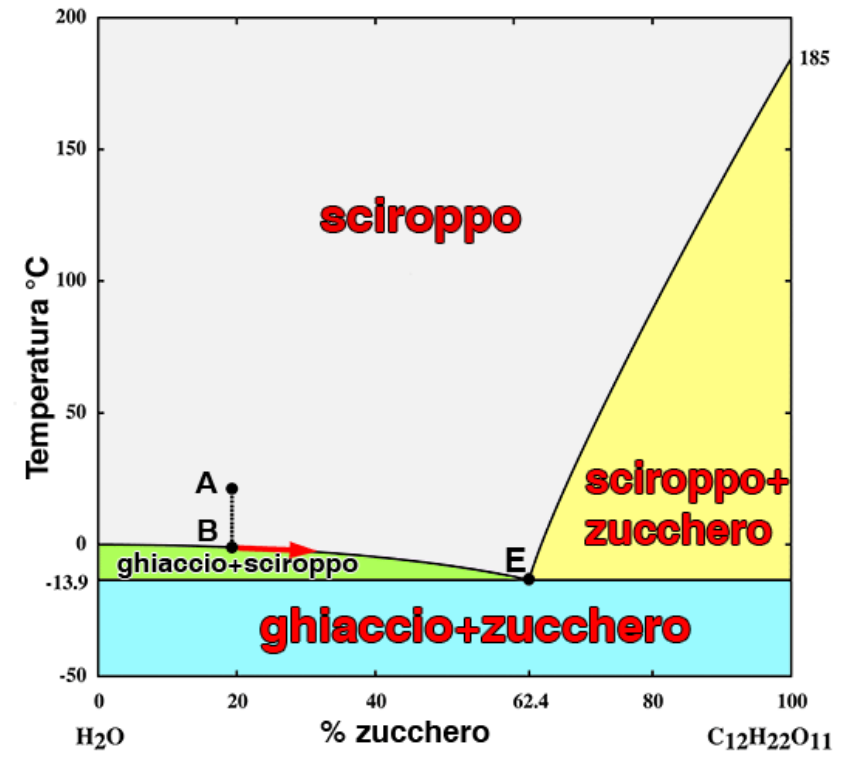
\includegraphics[width=10cm]{immagini/diagramma_di_stato_sciroppo.png}
\end{figure}

Avendo due componenti ricompare la frazione molare, perché possiamo avere infinite soluzioni al variare della composizione, quindi avremo la percentuale dei componenti in ascisse e la temperatura in ordinate.

Immaginiamo di avere una soluzione di acqua e il 20\% di zucchero (saccarosio) in massa.

Partiamo dal punto A che mostra questa composizione alla temperatura di 20° C. Raffreddiamo lentalmente, in modo da avere una successione di stati di equilibrio, fino a raggiungere gli 0° C. Se fosse stata acqua pura avremmo già del ghiaccio, ma non essendola questo non si forma. Abbassando ulteriormente la temperatura iniziano a formarsi i primi cristalli di ghiaccio (non di soluzione ghiacciata!), cioè si sta separando un po' di solvente che diventa solido.

Dato che stiamo togliendo solvente, la soluzione si sta concentrando, per cui per poter continuare ad avere la solidificazione dobbiamo continuare ad abbassare la temperatura, perché a una soluzione pià concentrata corrisponde una temperatura di congelamento più bassa.

La concentrazione aumenta e il punto di congelamento diminuisce fino al raggiungimento del punto E, che è detto \textbf{punto eutettico}: in tale punto la composizione del solido che si forma è uguale a quella della soluzione da cui si separa
\subsubsection{Diagramma di fase della salamoia}

\begin{figure}[htp]
    \centering
    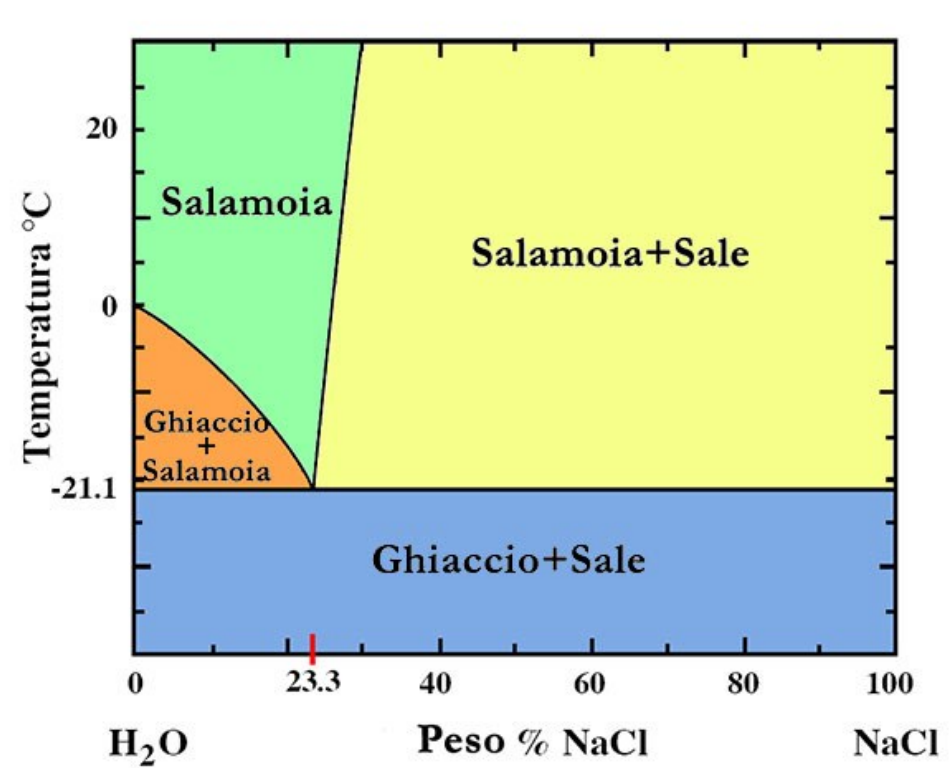
\includegraphics[width=10cm]{immagini/diagramma_di_stato_salamoia.png}
\end{figure}